\chapter{Implementation}

In this chapter, the theoretical explanations of the previous chapters are translated into practical implementations with Python.

\section{UDS implementation of the Scapy library}

First, to understand the later request generations for each service it is explained how to create UDS data with the Scapy library. And then, for completeness, how the data is transmitted.

\subsection{Create UDS data}

One of the core classes in Scapy is the \mintinline{python}{Packet} class. All definitions of network layers, such as Ethernet, IP, TCP, CAN, UDS and so on, are defined in a class inheriting from it, regardless of the layer level.

Its most important member is the \mintinline{python}{fields_desc} list. It is a requirement for each layer to overwrite it. Its elements must inherit from the \mintinline{python}{Field} class. The chosen field classes define the structure of each header field.

\begin{listing}[H]
\begin{minted}
[frame=single,
framerule=0pt,
framesep=2mm,
baselinestretch=1.2,
bgcolor=VeryLightGray,
fontsize=\footnotesize,
linenos]
{python}
class UDS(Packet):
    services = {
            0x10: 'DiagnosticSessionControl',
            # [...]
            0x22: 'ReadDataByIdentifier',
            # [...]
            0x7f: 'NegativeResponse'}
    fields_desc = [
        XByteEnumField('service', 0, services)
    ]
\end{minted}
\caption{Implementation of the root class for UDS in Scapy.}
\label{lst:uds-implementation}
\end{listing}

The UDS class (see \autoref{lst:uds-implementation}) contains only a \mintinline{python}{XByteEnumField} field. Field class names are composed of keywords.
\begin{samepage}
\begin{itemize}
    \item \textbf{X}: Represent its value as a hexadecimal value for the user.
    \item \textbf{Byte}: The field has 8-bits.
    \item \textbf{Enum}: The field expects a dictionary mapping from machine-readable values to human-readable texts.
\end{itemize}
\end{samepage}

\mintinline{python}{X} and \mintinline{python}{Enum} only affect the representation of the field. The \mintinline{python}{Byte} keyword is the only one here that defines the actual structure of the field.

This particular field are given three parameters:

\begin{itemize}
    \item \mintinline{python}{'service'}: The name of the field.
    \item \mintinline{python}{0}: The default value of the field.
    \item \mintinline{python}{services}: The dictionary mapping from machine-readable values to human-readable texts.
\end{itemize}

This field contains the Service Identifier (SID).

The Scapy implementation starts a new class whenever the subsequent fields depend on a field value of the current layer. This is the case here, since the next fields depend on the SID. The service specific fields are defined in their own classes, for example:

\begin{listing}[H]
\begin{minted}
[frame=single,
framerule=0pt,
framesep=2mm,
baselinestretch=1.2,
bgcolor=VeryLightGray,
fontsize=\footnotesize,
linenos]
{python}
class UDS_DSC(Packet):
    diagnosticSessionTypes = {
            # [...]
            0x03: 'extendedDiagnosticSession',
            # [...]
    }
    fields_desc = [
        ByteEnumField('diagnosticSessionType', 0,  diagnosticSessionTypes)
    ]

bind_layers(UDS, UDS_DSC, service=0x10)
\end{minted}
\caption{Implementation of the DSC service in Scapy.}
\label{lst:uds-dsc-implementation}
\end{listing}

The \mintinline{python}{bind_layers} call (line 11 of \autoref{lst:uds-dsc-implementation}) tells Scapy the relationship between the classes \mintinline{python}{UDS} and \mintinline{python}{UDS_DSC}. This information will be used by Scapy for building and dissecting data.
Then, if UDS data is received with the SID 0x10, it continues dissecting it with the field definitions of \mintinline{python}{UDS_DSC}. And vice versa, if \mintinline{python}{UDS_DSC} data is stacked on an \mintinline{python}{UDS} data for building, its SID field is automatically set to 0x10.

Layers are stacked with the division operator of python.

\begin{listing}[H]
\begin{minted}
[frame=single,
framerule=0pt,
framesep=2mm,
baselinestretch=1.2,
bgcolor=VeryLightGray,
fontsize=\footnotesize,
linenos]
{python}
uds_data = UDS() / UDS_DSC(diagnosticSessionType=0x03)
bytes(uds_data) # prints: 0x10 0x03
\end{minted}
\caption{Stacking \mintinline{python}{UDS} and \mintinline{python}{UDS_DSC} to a complete UDS request.}
\label{lst:uds-dsc-stacking}
\end{listing}

As can be seen, the SID of the UDS data is 0x10, although it was never explicitly set. Scapy set it because of the previous binding.


\subsection{Send UDS data with an ISO-TP socket}

There are two ISO-TP socket implementations in Scapy. A software and a native implementation. Until including Linux kernel 5.9, the corresponding ISO-TP module for Linux had to be installed separately \cite{isotp-module}. Since Linux kernel 5.10, it is part of the Linux mainline kernel \cite{isotp-commit}. Both implementations handle the ISO-TP data themselves, i.e. segmentation.

An ISO-TP socket contains a source and destination identifier. They have the same purpose as IP addresses. The source identifier (\mintinline{text}{sid}) is used for outgoing CAN frames, and the destination identifier (\mintinline{text}{did}) for incoming frames. In other words, the \mintinline{text}{sid} must contain the identifier to which the ECU expects requests, and the \mintinline{text}{did} must contain the identifier with which it responds. They must be known to be able to send requests to ECUs and receive their responses.

The usage of the native implementation is presented by the following code snippet:

\begin{listing}[H]
\begin{minted}
[frame=single,
framerule=0pt,
framesep=2mm,
baselinestretch=1.2,
bgcolor=VeryLightGray,
fontsize=\footnotesize,
linenos]
{python}
from scapy.contrib.isotp import ISOTPNativeSocket
socket = ISOTPNativeSocket('vcan0', sid=0x123, did=0x456)
uds_data = UDS() / UDS_DSC(diagnosticSessionType=0x03)
socket.send(uds_data)
\end{minted}
\caption{Sending UDS data with an ISO-TP socket.}
\label{lst:send-packet-isotp}
\end{listing}

The resulting frame and its response by the ECU can be observed with the \mintinline{text}{candump} program shown in \autoref{subsubsec:can-utils}. Line 2 of \autoref{lst:send-packet-isotp} defines \mintinline{text}{sid=0x123} and \mintinline{text}{did=0x456}. Thus, the request has the CAN identifier 0x123, and the response the expected CAN identifier 0x456. If the ECU responds with a different identifier, the response would not be received by this ISO-TP socket.

\begin{samepage}
\begin{minted}{text}
    $ candump vcan0
    vcan0  123   [3]  02 10 03
    vcan0  456   [7]  06 50 03 00 32 01 f4
\end{minted}
\end{samepage}

The request is explained step by step in the following list:

\begin{itemize}
    \item \mintinline{text}{0x123}: The CAN identifier.
    \item \mintinline{text}{[3]}: The length of the CAN payload.
    \item \mintinline{text}{0x02}: ISO-TP data showing the length of the layer 7 (UDS) payload.
    \item \mintinline{text}{0x10}: The SID of the DSC service.
    \item \mintinline{text}{0x03}: The parameter for the DSC service.
\end{itemize}

\section{Explaining the service enumerators of the UDS Scanner}

% TODO: Add that it was still work in progress while doing this work
% and thus, that problems occured and had to be fixed.
% Out of scope of this work.

Enumerators are service-specific and create all possible requests for a service.
For example, the enumerator of the DSC service is called \mintinline{python}{UDS_DSCEnumerator}. The most important member of these classes is the \mintinline{python}{_get_initial_requests} method. The return value is an iterable object which contains the requests for this service.

Each enumerator will be executed for each found state of the ECU. So, if an enumerator already was executed, and afterwards a new state is found by the UDS Scanner, this enumerator will be executed again within the same scan with the new-found state.

For a better understanding, the \mintinline{python}{UDS_DSCEnumerator} implementation will be described exemplary.

\begin{listing}[H]
\begin{minted}
[frame=single,
framerule=0pt,
framesep=2mm,
baselinestretch=1.2,
bgcolor=VeryLightGray,
fontsize=\footnotesize,
linenos]
{python}
class UDS_DSCEnumerator(UDS_Enumerator, StateGenerator):
    def _get_initial_requests(self, **kwargs):
        session_range = kwargs.pop('session_range', range(2, 0x100))
        return UDS() / UDS_DSC(diagnosticSessionType=session_range)
\end{minted}
\caption{Implementation of the enumerator scanning the DSC service.}
\label{lst:dsc-enumerator}
\end{listing}

The method can be configured by keyword parameters. The only one read by this method implementation is \mintinline{python}{session_range}. If none is given, which is usually the case, it defaults to the range from 0x02 to 0xff. So, this enumerator creates 254 requests for each state by default. It is also a \mintinline{python}{StateGenerator}, which means its requests can change the state of the ECU (see \autoref{subsec:states}). This is detected by the UDS Scanner and the new state will be scanned as well.

Enumerators can output their results as a text-table. For example a possible output of the UDS enumerator is:

\begin{samepage}
\begin{minted}[fontsize=\footnotesize]{text}
----------+--------------------------+--------------------------+--------------------------+
          | defaultState             | state2                   | state3                   | 
----------+--------------------------+--------------------------+--------------------------+
0x02      | PR: Supported            | NR: conditionsNotCorrect | PR: conditionsNotCorrect | 
0x03      | NR: conditionsNotCorrect | PR: Supported            | PR: conditionsNotCorrect | 
0x82      | NR: conditionsNotCorrect | NR: conditionsNotCorrect | -                        | 
----------+--------------------------+--------------------------+--------------------------+
\end{minted}
\end{samepage}

Each row is a request. Here are listed requests of the DSC service with parameters 0x02, 0x03 and 0x82. Each column is a state. And each cell shows the response for each request per state (PR = positive response, NR = negative response).

A PenTester would be able to extract a state machine from this table (see \autoref{fig:state-machine-of-scan}).

\begin{figure}[H]
    \centering
    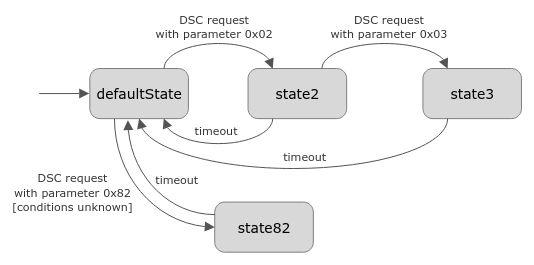
\includegraphics[width=0.68\textwidth]{state-machine-of-scan}
    \caption{Partial result for a PenTester of a UDS scan.}
    \label{fig:state-machine-of-scan}
\end{figure}

So-called staged enumerators contain enumerators where each enumerator is a stage. They start executing the first enumerator for each state, followed by each subsequent enumerator in the same way. For example:
\begin{enumerate}
    \item enumerator1 : state1
    \item enumerator1 : state2
    \item enumerator2 : state1
    \item enumerator2 : state2
\end{enumerate}

For each stage transition connectors can be defined. They are functions with two arguments, containing the previous enumerator and the new enumerator. Here, the results of the previous enumerator can be evaluated and the next enumerator can be configured accordingly. The connector will be automatically called by the UDS Scanner and expects a dictionary as return value that will be passed to the next enumerator. 

\begin{listing}[H]
\begin{minted}
[frame=single,
framerule=0pt,
framesep=2mm,
baselinestretch=1.2,
bgcolor=VeryLightGray,
fontsize=\footnotesize,
linenos]
{python}
class MyStagedEnumerator(StagedAutomotiveTestCase):
    @staticmethod
    def connector_stage1_stage2(stage1_enum, stage2_enum):
        results = stage1_enum.get_results()
        stage2_config = create_config(results)
        return stage2_config
    
    def __init__(self):
        super().__init__(
            [Stage1Enumerator(), Stage2Enumerator()],
            connectors=[None, self.connector_stage1_stage2])
\end{minted}
\caption{Example implementation of a staged enumerator.}
\label{lst:staged-enumerator}
\end{listing}

\section{Implementing new enumerators for the RC service}

Three classes are of interest:

\begin{itemize}
    \item \mintinline{python}{RCEnumerator}: Defaults to scanning the whole RC service, including all three types.
    \item \mintinline{python}{RCStartEnumerator}: Only scanning type1 of the RC service.
    \item \mintinline{python}{RCSelectiveEnumerator}: Staged enumerator containing an RCStartEnumerator and an RCEnumerator.
\end{itemize}

For this work, the configurability of the \mintinline{python}{RCEnumerator} was improved, and the \mintinline{python}{RCStartEnumerator} and \mintinline{python}{RCSelectiveEnumerator} was created. \autoref{fig:rc-schematic} gives a first overview of the new implementation mechanisms.

\begin{figure}[htb]
    \centering
    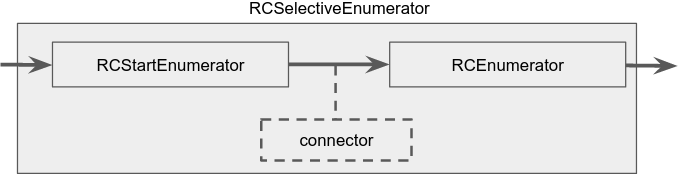
\includegraphics[width=0.7\textwidth]{rc-schematic}
    \caption{Schematic illustration of the new \mintinline{python}{RCSelectiveEnumerator}.}
    \label{fig:rc-schematic}
\end{figure}

First, the \mintinline{python}{RCEnumerator} will be explained by having a closer look at its \mintinline{python}{_get_initial_requests} method.

\begin{listing}[H]
\begin{minted}
[frame=single,
framerule=0pt,
framesep=2mm,
baselinestretch=1.2,
bgcolor=VeryLightGray,
fontsize=\footnotesize,
linenos]
{python}
class UDS_RCEnumerator(UDS_Enumerator):
    def _get_initial_requests(self, **kwargs):
        type_list = kwargs.pop("type_list", [1, 2, 3])
        scan_range = kwargs.pop("scan_range", range(0x10000))

        return (
            UDS() / UDS_RC(routineControlType=rc_type,
                           routineIdentifier=data_id)
            for rc_type, data_id in itertools.product(type_list, scan_range)
        )
\end{minted}
\caption{The extended enumerator for the RC service.}
\label{lst:rc-enumerator}
\end{listing}

Two parameters can be configured, the \mintinline{python}{type_list} and \mintinline{python}{scan_range}. Both default to the values required to scan the whole RC service. Eventually, the method returns a generator that generates all requests possible by pairing the values of \mintinline{python}{type_list} and \mintinline{python}{scan_range}. This accomplishes the \mintinline{python}{itertools.product} method from the Python Standard library. It returns the cartesian product of the input iterables.

Next, the \mintinline{python}{RCStartEnumerator}.

\begin{listing}[H]
\begin{minted}
[frame=single,
framerule=0pt,
framesep=2mm,
baselinestretch=1.2,
bgcolor=VeryLightGray,
fontsize=\footnotesize,
linenos]
{python}
class UDS_RCStartEnumerator(UDS_RCEnumerator):
    def _get_initial_requests(self, **kwargs):
        kwargs["type_list"] = [1]
        return super()._get_initial_requests(**kwargs)
\end{minted}
\caption{The enumerator for the RC service scanning only type1.}
\label{lst:rc-start-enumerator}
\end{listing}

Its \mintinline{python}{_get_initial_requests} method is simple. It fixes the \mintinline{python}{type_list} to type1 and then calls its implementation of the super class, which is the previously explained \mintinline{python}{UDS_RCEnumerator}. This results in generating requests only for type1.

The \mintinline{python}{UDS_RCSelectiveEnumerator} connects both of these enumerators.

\begin{listing}[H]
\begin{minted}
[frame=single,
framerule=0pt,
framesep=2mm,
baselinestretch=1.2,
bgcolor=VeryLightGray,
fontsize=\footnotesize,
linenos]
{python}
class UDS_RCSelectiveEnumerator(StagedAutomotiveTestCase):
    expansion_width = 253

    @staticmethod
    def connector_start_to_full(rc_start, rc_full):
        identifiers_with_pr = [r.resp.routineIdentifier for r
                            in rc_start.results_with_positive_response]

        scan_range = points_to_ranges(
            identifiers_with_pr, UDS_RCSelectiveEnumerator.expansion_width)

        return {"type_list": [2, 3],
                "scan_range": scan_range}

    def __init__(self):
        super().__init__(
            [UDS_RCStartEnumerator(), UDS_RCEnumerator()],
            [None, self.connector_start_to_full])
\end{minted}
\caption{The staged enumerator combining the start and complete enumerator for the RC service.}
\label{lst:rc-selective-enumerator}
\end{listing}

This staged enumerator has the \mintinline{python}{RCStartEnumerator} as the first stage, and the \mintinline{python}{RCEnumerator} as the second and last stage.
The expansion width is fixed to \textbf{253} as it was elaborated in \autoref{subsubsec:rc-elaborating}.

The connector calls \mintinline{python}{points_to_ranges} to expand the found identifiers of the first stage to ranges and passes them to the second stage. In addition, the connector configures the \mintinline{python}{RCEnumerator} to scan only type2 and type3, since type1 should no longer be scanned.

\begin{listing}[H]
\begin{minted}
[frame=single,
framerule=0pt,
framesep=2mm,
baselinestretch=1.2,
bgcolor=VeryLightGray,
fontsize=\footnotesize,
linenos]
{python}
def points_to_ranges(points, expansion_width):
    generators = []
    for identifier in points:
        start = max(identifier - expansion_width, 0)
        end = min(identifier + expansion_width + 1, 0x10000)
        generators.append(range(start, end))
    ranges_with_overlaps = itertools.chain.from_iterable(generators)
    return sorted(set(ranges_with_overlaps))
\end{minted}
\caption{Function extending points to ranges.}
\label{lst:points-to-ranges}
\end{listing}

\mintinline{python}{points_to_ranges} expands points to ranges and also resolves any overlaps to a continuous range.
First, a range generator is created for each given point. Then, they are chained and converted to a set, removing potential overlaps. This set is sorted in a list, to ensure understandable candump logs of a scan.

\section{Implementing new enumerators for the RDBI service}

Again, three classes are of interest:

\begin{itemize}
    \item \mintinline{python}{RDBIEnumerator}: Defaults to scanning the whole RDBI service.
    \item \mintinline{python}{RDBIRandomEnumerator}: Scanning block-based with random identifiers.
    \item \mintinline{python}{RDBISelectiveEnumerator}: Staged enumerator containing an RDBIRandomEnumerator and an RDBIEnumerator.
\end{itemize}

The new implementation is two-staged. First, the \mintinline{python}{RDBIRandomEnumerator} is executed. Then, the connector creates requests for whole blocks, if any of their requests were answered positively, and ensured that for a single block each identifier is queried only once. The resulting requests are passed to the configurable \mintinline{python}{RDBIEnumerator}. \autoref{fig:rdbi-schematic} shows that schematically.

\begin{figure}[htb]
    \centering
    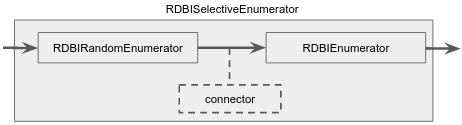
\includegraphics[width=0.7\textwidth]{rdbi-schematic}
    \caption{Schematic illustration of the new \mintinline{python}{RDBISelectiveEnumerator}.}
    \label{fig:rdbi-schematic}
\end{figure}

The explanation starts with the original enumerator, here the \mintinline{python}{RDBIEnumerator}.

\begin{listing}[H]
\begin{minted}
[frame=single,
framerule=0pt,
framesep=2mm,
baselinestretch=1.2,
bgcolor=VeryLightGray,
fontsize=\footnotesize,
linenos]
{python}
class UDS_RDBIEnumerator(UDS_Enumerator):
    def _get_initial_requests(self, **kwargs):
        scan_range = kwargs.pop("scan_range", range(0x10000))
        return (UDS() / UDS_RDBI(identifiers=[x]) for x in scan_range)
\end{minted}
\caption{The enumerator scanning the whole RDBI service by default.}
\label{lst:rdbi-enumerator}
\end{listing}

Since the RDBI service has only one parameter, its \mintinline{python}{_get_initial_requests} remains simple, generating RDBI requests for identifiers from 0 to 65,535, if not configured otherwise.

Implementing the \mintinline{python}{RDBIRandomEnumerator} was a challenge because it must include the probabilities of positively responded identifiers for each block. With a block size of \textbf{64} (see \autoref{subsubsec:rdbi-behavior}), there would need to be a list with $\frac{2^{16}}{64} = 1024$ elements. Thus, it is desirable to represent this information more compactly. A better representation is based on two facts. That the probabilities are ultimately converted to the number of samples, and that at least one request should be generated for each block. For the former, the number of samples for each block were pre-computed instead of being computed at runtime. This simplifies the list in the sense that integers are stored instead of float values. Second, the number of samples is not stored for all blocks, but only for blocks whose number of samples is greater than or equal to two. And blocks for which no value is stored, the value one is used. This automatically solves that each block is probed with at least one request, even if its probability is 0\,\%. These simplifications transformed the list of 1024 elements into a dictionary of only 109 elements. The non-simplified version is shown in \autoref{app:random-not-compact}.

\begin{listing}[H]
\begin{minted}
[frame=single,
framerule=0pt,
framesep=2mm,
baselinestretch=1.2,
bgcolor=VeryLightGray,
fontsize=\footnotesize,
linenos]
{python}
class UDS_RDBIRandomEnumerator(UDS_RDBIEnumerator):
    def _get_initial_requests(self, **kwargs):
        samples_per_block = {
            4: 29, 5: 22, 6: 19, 8: 11, 9: 11, 10: 13, 11: 14,
            # [...]
            1013: 14, 1014: 15
        }
        to_scan = []
        block_size = UDS_RDBIRandomEnumerator.block_size
        for block_index, start in enumerate(range(0, 2 ** 16, block_size)):
            end = start + block_size
            count_samples = samples_per_block.get(block_index, 1)
            to_scan += random.sample(range(start, end), count_samples)

        positive_identifiers = [t.resp.dataIdentifier for t in
                                self.results_with_positive_response]
        to_scan += positive_identifiers

        to_scan = sorted(list(set(to_scan)))
        return (UDS() / UDS_RDBI(identifiers=[x]) for x in to_scan)
\end{minted}
\caption{The enumerator scanning randomly the RDBI service based on blocks.}
\label{lst:rdbi-random-enumerator}
\end{listing}

The \mintinline{python}{random.sample} function from the Python Standard library returns a list of given length with unique elements chosen from the given sequence.

The implementation exploits the observation that most identifiers are available in multiple states. Thus, the randomly generated identifiers are appended with the identifiers that were answered positively in any previous state.

Again, the \mintinline{python}{UDS_RDBISelectiveEnumerator} brings these two enumerators together.

\begin{listing}[H]
\begin{minted}
[frame=single,
framerule=0pt,
framesep=2mm,
baselinestretch=1.2,
bgcolor=VeryLightGray,
fontsize=\footnotesize,
linenos]
{python}
class UDS_RDBISelectiveEnumerator(StagedAutomotiveTestCase):
    block_size = 2 ** 6

    @staticmethod
    def connector_random_to_sequential(rdbi_random, rdbi_full):
        identifiers_with_pr = \
            [r.resp.dataIdentifier
            for r in rdbi_random.results_with_positive_response]

        scan_range = points_to_blocks(
                identifiers_with_pr,
                UDS_RDBISelectiveEnumerator.block_size)
        return {"scan_range": scan_range}

    def __init__(self):
        super().__init__(
            [UDS_RDBIRandomEnumerator(), UDS_RDBIEnumerator()],
            [None, self.connector_random_to_sequential])
\end{minted}
\caption{The staged enumerator combining the random and complete enumerator for the RDBI service.}
\label{lst:rdbi-selective-enumerator}
\end{listing}

Since it is similar to the \mintinline{python}{RCSelectiveEnumerator}, it will not be explained any further. Only the \mintinline{python}{points_to_blocks} will be described in more detail.

\begin{listing}[H]
\begin{minted}
[frame=single,
framerule=0pt,
framesep=2mm,
baselinestretch=1.2,
bgcolor=VeryLightGray,
fontsize=\footnotesize,
linenos]
{python}
def points_to_blocks(points, block_size):
    generators = []
    for start in range(0, 2 ** 16, block_size):
        end = start + block_size
        pr_in_block = any((start <= identifier < end
                        for identifier in points))
        if pr_in_block:
            generators.append(range(start, end))
    scan_range = itertools.chain.from_iterable(generators)
    return scan_range
\end{minted}
\caption{Function extending points to fixed blocks.}
\label{lst:points-to-blocks}
\end{listing}

Unlike \mintinline{python}{points_to_ranges}, its block boundaries are fixed. It traverses each block and checks if any of the given identifiers is part of that block. If this is the case, the block will be scanned completely.

Unfortunately, this can lead to double-scanned identifiers, since instead of scanning only the remaining identifiers that have not yet been scanned in the respective blocks, the entire blocks are rescanned. Although an attempt was made to implement this, the UDS scanner does not provide the necessary interfaces to do so. The connectors only know the enumerators, but not the currently executed state. However, this is necessary to check which identifiers have already been scanned in the random enumerator for the current state. Nevertheless, the number of duplicate requests is low, so the request savings hardly decrease.

\section{Extending the enumerators to skip unsupported services}

In contrast to the previous approaches, this one is not applied to specific service enumerators, but to their super class. It evaluates each response, for example to detect if a new state was found. Here, a check was added for negative responses if they have an NRC of 0x11 or 0x7f. If they do, the enumerator is set to completed for the currently executed state.

\begin{listing}[H]
\begin{minted}
[frame=single,
framerule=0pt,
framesep=2mm,
frame=single,
framerule=0pt,
framesep=2mm,
baselinestretch=1.2,
bgcolor=VeryLightGray,
fontsize=\footnotesize,
linenos]
{python}
class AutomotiveTestCase(AutomotiveTestCaseABC):
    """Base class for Enumerators"""

    def _evaluate_response(self, response, **kwargs):

        # Removed code for simplification

        if exit_if_service_not_supported and response.service == 0x7f:
            response_code = self._get_negative_response_code(response)
            if response_code in [0x11, 0x7f]:
                # execute of current state is completed,
                # since a serviceNotSupported NR was received
                current_state = self._results[-1].state
                self._state_completed[current_state] = True
                # stop current execute and exit
                return True

        # Removed code for simplification

        return False
\end{minted}
\caption{The extended super class of each enumerator with skipping unsupported services.}
\label{lst:enumerator-super-class}
\end{listing}    
